\chapter{Heritage of ice reservoirs}

\cleanchapterquote{Before the artificial glacier, we struggled to get any barley. But now we can grow many
	crops, even potatoes, which need to be planted earlier in the spring, but sell for much more money.
}{Tashi Tundup}{(A 76-year-old farmer in Ladakh, India)}

Climate warming has resulted in the retreat and thinning of mountain glaciers
\citep{ipccCrossChapterPaperMountains2022}. This has implications for water availability in river basins with considerable glacierized areas in their headwaters, such as \ac{HMA}. Glaciers in \ac{HMA} provide an important
gradual release of water that is used by many people locally and downstream for irrigation, drinking water, and
hydropower. Climate change in this densely populated region can have serious consequences for glacier meltwater
supply to the rivers \citep{immerzeelImportanceVulnerabilityWorld2020}. In this context, the development of
water storage technologies is crucial to ensure continued sustenance of cryosphere-fed irrigation networks.

People in mountains have a history of developing nature-based solutions to live in a dangerous and dynamic
environment, which will be invaluable to learn from for future adaptation and mitigation measures. One such
technology developed by communities in Ladakh are \ac{AIRs}. These strategies involve augmenting their glacial
ice reservoirs with human-made ones that provide supplementary irrigation during the spring.

\begin{figure}[htb]
	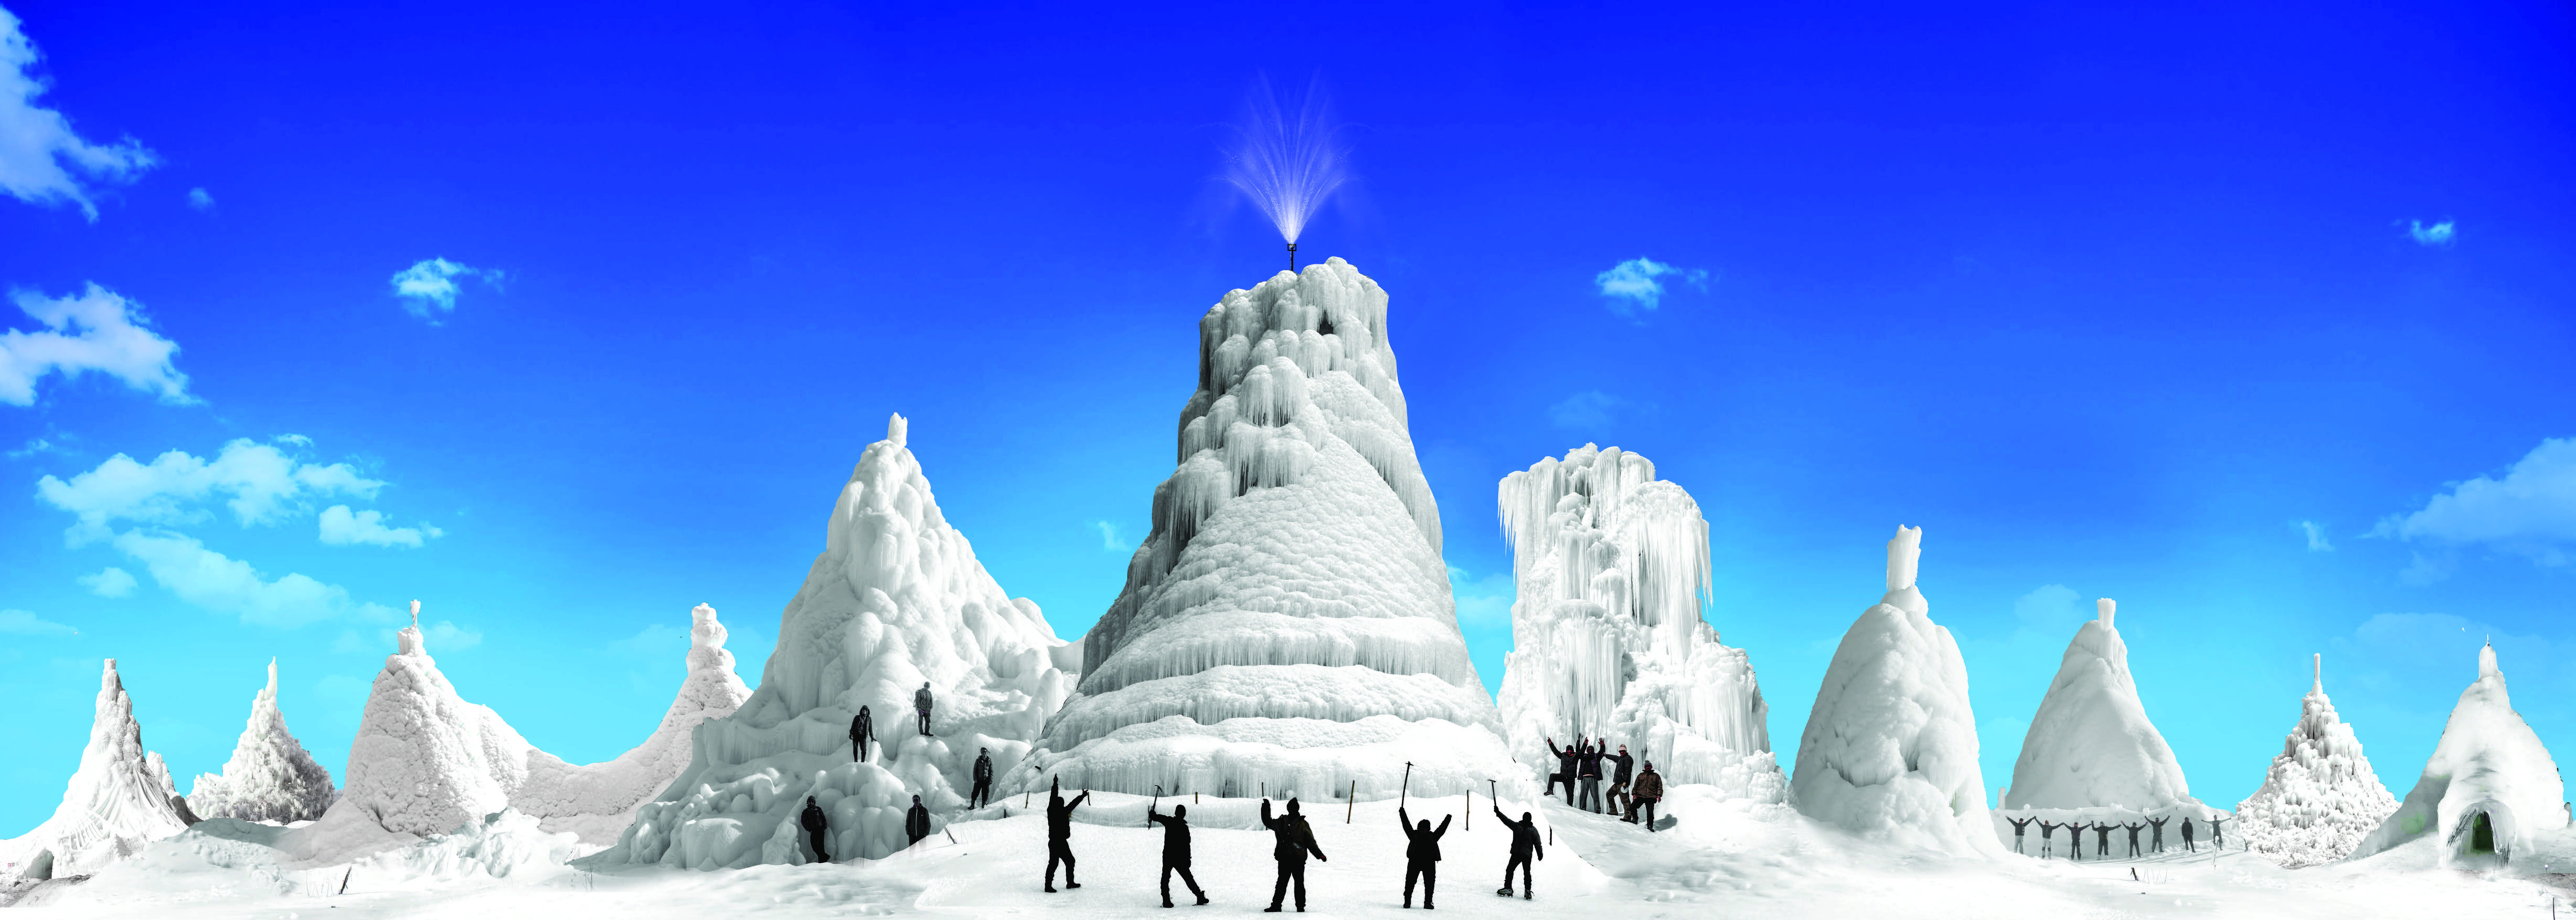
\includegraphics[width=\textwidth]{figs/AIRs_Ladakh}
	\caption{Compilation of AIRs built in different villages in Ladakh.}
	\label{fig:airs_ladakh}
\end{figure}

Although such technologies have attracted renewed attention as strategies to increase water security, the scientific evidence about their potential hydrological contributions is still limited. AIR observations and investigations
date back to the mid-2000s \citep{tveitenGlacierGrowingLocal2007}. The vast majority of these have been published in the
2010s, mostly using qualitative methods. Due to the small-scale processes, complex feedbacks, and nonlinearities
governing their evolution, modelling volume evolution of ice stupas is difficult and only feasible if supported
by comprehensive datasets. Recent advances in glacial models and drones provide the opportunity to quantify
these surface processes using high-resolution data on volume changes of \ac{AIRs}. The main objective of the present
thesis is therefore \textit{to increase the understanding of volume dynamics of \ac{AIRs} to provide tools
that reduce their water losses and maintenance requirements}, with a specific focus on the potential application
of glacial models. This is achieved by focusing on the following two specific research questions:

\begin{enumerate}
  \item{What is the influence of construction location and fountain characteristics on ice stupa volume
    evolution?}
  \item{How can ice stupa fountain systems be engineered to reduce water losses and maintenance efforts?}
\end{enumerate}

In this chapter, the main findings are discussed and integrated in a broader perspective. The limitations in the
methodology used are pointed out, and recommendations are provided for upscaling AIR water storage technology.

\section{Recommendations and challenges}

The studies presented in this thesis provide insights into the volume evolution of \ac{AIRs}. However, various research gaps still remain and need to be overcome before \ac{AIRs} can be integrated into water resource
management plans. Moreover, further development of the construction tools is required to improve the
cost-effectiveness, size, and survival duration of \ac{AIRs}. However, development and application of
nature-based solutions such as \ac{AIRs} are not possible without extensive collaboration. In this context,
specific recommendations and major challenges that scientists, engineers, and farmers can solve together are laid
out below:

\subsection{For scientists}
% \subsection{To improve scientific data and model approaches}

Scientists can contribute through development of the software tools in the automation system, identification of
other favorable construction regions, and integration of nature-based water storage technologies in water
resource management plans. All these require customization of the models introduced in the
\textit{Science} chapter. Specifically, use of the COSISTUPA model is indicated for future estimations of AIR
volume. This model needs to be extended so that it can account for future climate variability and produce
accurate meltwater predictions. Modelling the future is fundamentally different from simulating the past: for the
past, the model serves as a tool for interpreting and best exploiting field measurements---and can be directly
constrained by them; for the future, climate variability must be comprehended to be able to yield realistic
projections. Almost all methodological steps in the modelling of future AIR runoff are subject to potential
enhancements. Model accuracy can be enhanced with the following methods:

\subsubsection{Quality and quantity of calibration and validation datasets}

The methodology used to acquire the radius, area, and volume of \ac{AIRs} (Appendix \ref{sec:drone_method}) from
each drone survey presents several drawbacks. The calibration and validation processes used present inherent temporal
and spatial biases due to the following subjective choices:

\begin{itemize}
	\item \textbf{Number and timing of drone surveys}. For example, among the five surveys of the IN21 AIR, most of them were
	      conducted around early March, when the AIR volume was near its maximum, whereas the seven surveys of the CH21
	      location were more evenly spaced out. This observation bias responds to logistical issues
	      in conducting measurements at regular intervals.

  \item \textbf{The meteorological conditions under which surveys are performed.} In particular, precipitation
    events reduce \ac{DEMs} quality, since they create uniform snow surfaces over \ac{AIRs}. These surfaces do
    not allow the identification of features that can be used to extract the radius and area of the \ac{AIRs}.

\end{itemize}

Thus, the quality of volume validation is limited by the high uncertainties of the drone processing
methodology. This limitation can be overcome by extending the model validation set using two measurement
approaches. First, measuring daily AIR meltwater quantities; accuracy of this validation method
depends on the wind speeds of the location but can be improved if the terrain is made waterproof and oriented so
that most of the AIR runoff can be collected. Second, conducting \ac{GPR} surveys; \ac{GPR} is
sensitive to subtle changes in the properties of ice layers, making it a powerful tool to image the internal
structure of ice structures. The basic principle of a pulsed \ac{GPR} system is to send an electromagnetic
signal into the ground and to record the signal reflections as a function of their two-way travel time. Partial
reflections of the electromagnetic wave recorded as internal reflection horizons (IRH) occur at vertical
discontinuities in the dielectric material. From polar studies, IRH are known to coincide with variations in
density and liquid water content \citep{forster2014extensive}. Therefore, \ac{GPR} can be a crucial method to
calibrate and validate spatial density and volume variations of \ac{AIRs}.


\begin{figure}[htb]
  \centering
	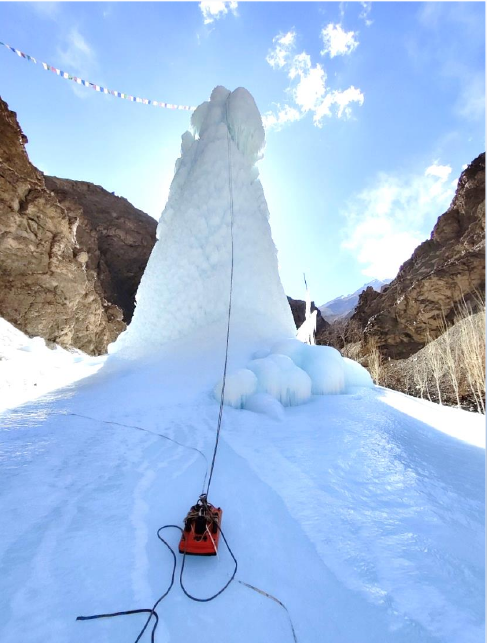
\includegraphics[width=8 cm]{figs/gpr_survey}
  \caption{Portable \ac{GPR}s carried across the surface of \ac{AIRs} to produce the associated datasets.
    (Photo: Shijay Projects)}
	\label{fig:gpr_survey}
\end{figure}

Although \ac{GPR} surveys were conducted on four ice stupas in March, 2020 (Fig. \ref{fig:gpr_survey}),
these datasets remain unused. They can be downloaded at \citet{balasubramanian_suryanarayanan_2022_7056646}.

\subsubsection{Albedo parametrization}

The albedo parametrization illustrated by equation \ref{eqn:alb} had to be modified to accomodate fountain
discharge events. Little knowledge is available to understand the decay of albedo due to such events. Therefore,
a simplistic approach of increasing the decay rate by a constant factor was chosen. However, the value of this
factor has no basis on measurements. Field-based albedo measurements are required to better
parametrize the effect of water spray on the surface albedo decay rate.

\subsubsection{Turbulent heat flux parametrization}

The method used to calculate turbulent heat fluxes by \citet{garrattAtmosphericBoundaryLayer1992} assumes that
these fluxes act over a uniform planar surface. This leads to the use of a exposure/roughness parameter
$\mu_{cone}$ as a correction factor. However, equation \ref{eqn:mu} about $\mu_{cone}$ is just an
educated guess. To base estimates of this parameter on information in literature is difficult. Many studies
have been performed on the effects of obstacles on atmospheric boundary layer flow (e.g., trees), but always in
an ensemble setting, focusing on the bulk effect of an ensemble of obstacles. In this thesis, the case is that of a single
obstacle in open terrain, and the roughness of the surface and the exposure are likely to lead to
larger turbulent fluxes.

\subsubsection{Spray radius quantification}

All models require the fountain spray radius as input. This is a significant limitation, since
these models are very sensitive to the spray radius parameter. Moreover, spray radius is not only determined by
fountain characteristics but also by wind-driven redistribution, refreezing, and melting events across
the AIR perimeter. The same fountain was observed to produce different spray radius values corresponding to different
winters for the Swiss experiments. Further discussion on this can be found in Section \ref{sec:interannual}.

\subsubsection{Quantification and development of ice terraces}

Although this thesis focuses on ice stupas, their ice volumes pale in comparison with ice terraces
\citep{nusserSociohydrologyArtificialGlaciers2019}. This is because ice stupas are limited by their fountain's
spray radius. However, ice terraces have no such limitations. Their thickness is only limited by the water
supply rate or meteorological conditions and they can occupy any construction area provided. However, ice stupas
are the preferred method of ice harvesting due to their longer survival duration and reduced construction
effort.

With a suitable redesign of the automation hardware, automated construction strategies can also be applied on
ice terraces. Such a construction strategy can potentially compound their size every consecutive winter with
minimal maintenance requirements. Therefore, future research direction should aim to answer the following
questions:

\begin{itemize}

	\item How can ice terrace construction systems be engineered to reduce their water losses and maintenance
	      efforts?

\end{itemize}

The methodology developed in this thesis should also apply for such an analysis.

\subsubsection{Adaptation potential of glacierized catchments with AIRs}

Vanishing glaciers, natural hazards (like inundations, mudflows, and landslides), decreasing river discharge,
drying springs, next to shifts in precipitation patterns are apparent climate change impacts which affect
glacierized catchments.

In the Peruvian Andes, both water scarcity (low-flow water risk) and glacial lake outburst floods (high flow
water risks) could have important impacts on local population, infrastructure and economic activities
\citep{motschmannIntegratedAssessmentsWater2020}. For example, the estimated loss in annual wheat output due to
reduced glacial runoff would be to the tune of 18 million USD even in the low emission scenario of Quillcay
catchment of Peru \citep{motschmannLossesDamagesConnected2020}. Similarly, in the Stok catchment of Ladakh,
glacial ice reserves have shrunk by more than 18 \% in the past 16 years, leading to a decline in crop
productivity \citep{sohebSpatiotemporalQuantificationKey2022}.

\ac{AIRs} can already buffer against low flow water risks in certain catchments. For example, ice terraces in
nearby valleys have been measured by \citet{nusserSociohydrologyArtificialGlaciers2019} with areas up to 19 \%
of the Stok glacier (0.8 $km^2$). With further technology development, \ac{AIRs} can also be used to mitigate high
flow water risks. The glacial lakes of the Andes and Himalayas can be siphoned to form AIRs at scales that last
perpetually. Such \ac{AIRs} can compound over the years to become another source of perennial water supply for the
respective catchments.

\subsection{For engineers}
% \subsection{To improve hardware tools}

The \textit{Technology} chapter shows one strategy that can improve the water-use efficiency of \ac{AIRs}. We chose
this strategy because it enables the use of the \ac{AIR} model in a simple and effective manner. However, all these
construction strategies are limited by the tools they use, namely the fountain and the pipeline. As scientists,
our methodology was not suitable to quantify and optimise these hardware tools. Below we discuss why this was
the case and provide some recommended methodologies to improve them:

\subsubsection{Fountain optimisation}

Contrary to the model assumptions, the parameters used to define the fountain were not independent. The fountain
height, aperture diameter, discharge rate, water temperature and spray radius were related through the
trajectories of the water droplets. The fountain nozzle design is crucial for increasing the ice volume
obtained. It determines the diameter of the water droplets and the angle of launch for their projectile motion.
The choice of these two parameters determines the rate of nuclueation process, pressure losses and discharge
rate ranges. For example, during the IN21 experiment, snow formation was observed, indicating that the fountain
water droplets have the potential to freeze before deposition on the AIR surface. In the CH22 experiment, the
higher aperture diameter of the non-scheduled fountain nozzle (Fig. \ref{fig:autovsman}) produced bigger droplets
and, therefore, had a lower fountain pressure loss when compared to the scheduled fountain. However, fountains
with large aperture diameters lose their ability to form water droplets at low discharge rates. Therefore, the
scheduled fountain nozzle design was used since it was able to produce water droplets with discharge rates as
low as 2 $l/min$.

However, no methodology currently exists to rank the different fountain nozzles used for construction. Quantifying
processes influenced by the fountain nozzle is challenging as it would require modelling the conduction,
convection, wind redistribution, and nucleation processes that droplets of varying diameters undergo during
their flight time. Instead, controlled experiments comparing the freezing rates between different fountain
diameters have a better chance to yield insights on the engineering design of fountain nozzles.

\subsubsection{Pipeline optimisation}

An ideal pipeline configuration could make this technology cheaper and maintenance free. However, optimization
of the pipeline material and diameters is yet to be performed---despite the time lost on pipeline freezing
events and the potential cost reduction with cheaper pipeline materials and sizes. Larger pipeline diameters
reduce the occurence of pipeline freezing events but increase the cost dramatically. In Ladakh, pipeline
diameters used have a wide range (from 0.03 to 0.3 $m$) since the choice of pipeline diameter also depends on
the additional insulation provided and whether or not it is buried. Therefore, a comprehensive cost-benefit
analysis of different combinations of insulation and pipeline materials is required to determine the optimum
design of the insulated pipeline system.

\subsubsection{Cost reduction of automation system}

Our strategy is not yet suitable for application in current AIR construction sites due to the cost of the
automation system (around 8,000 USD). However, we believe upto 10 fold cost reduction is possible through
simpler automation systems which control only the duration of fountain spray and not their quantity. 

% \subsection{To improve hardware tools}
\subsection{For farmers}

Farmers in Hindu Kush Himalayas have been improving ice harvesting technologies for generations as documented in
the \textit{Religion} chapter. But these technologies can also be leveraged by farmers in many other regions. In
the absence of an objective global-scale estimation of AIR water storage, we suggest some subjective guidelines
that can help narrow down favourable construction sites. Later, we illustrate the impact the automation system
can create in upscaling irrigation water supply in a mountain catchment of Ladakh.

\subsubsection{Metrics to judge site suitability}

We propose two sets of guidelines to identify future construction sites at a regional and a local scale. These
suggestions are guided by the different case studies presented in this thesis and field experiences in
Ladakh over the past six winters.

\textbf{Regional scale}

\begin{enumerate}

	\item Minimum median monthly temperature less than $0 \degree C$ to ensure sufficient freezing rate.
	\item Water supply with median discharge rate more than $2\, l/min$ to ensure sufficient water supply.

\end{enumerate}

\textbf{Local scale}

Given a valley or a region satisfying the above requirements, further selection of sites around the particular
water supply can be performed using the criterions below:

\begin{enumerate}
	\item Higher water source temperature to minimise risk of pipeline freezing events.
	\item Terrain slope between water source and site greater than 20 m every km to ensure sufficient
    gravitational head for fountain operation.
	\item Low daylight hours to decrease solar radiation induced melt.
	\item Higher altitude for higher freezing rates.
\end{enumerate}

\subsubsection{New ways to upscale irrigation water supply}

In this section, two hypothetical ice stupa construction scenarios namely, present and future are described. The
present scenario is a depiction of the construction efforts based on oral interviews and field experience. The
future scenario is a depiction of how the automation system developed in the \textit{Technology}
chapter can transform current construction
efforts. The objective of both the scenarios is to maximize the meltwater available for irrigation. Both these
scenarios are motivated by the construction campaigns conducted in the Gangles valley of Ladakh during the
winter of 2019/20 (Fig. \ref{fig:icestupa_valley}). This is the same valley where the IN21 study site was
located enabling us to extrapolate some of the freezing rates and ice volume estimations from
paper I. We conservatively assume that the valley had a
total water supply of around $120\,l/min$, a winter duration of 4 months and the fountain was operational for
only 8 hours per day for both the scenarios. 

\begin{figure}[htb]
	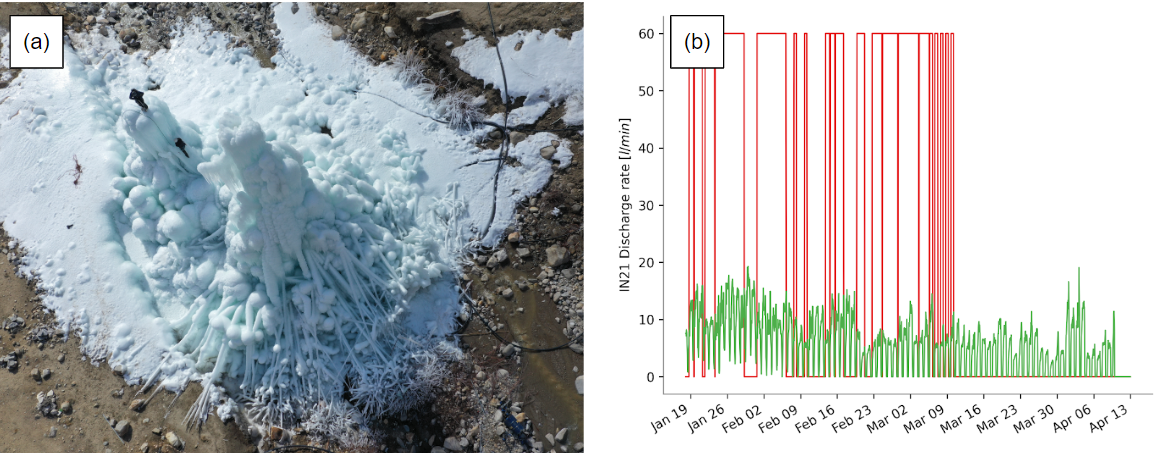
\includegraphics[width=\textwidth]{figs/gangles_data}

  \caption{(a) The IN21 ice stupa is a good example of the typical construction scenario (Photo: Norboo
  Thinles). (b) Its observed fountain discharge rate (red line) was interrupted several times due to pipeline
freezing events. The discharge quantities used were also much higher than the estimated freezing rate (green
line). }

	\label{fig:gangles_data}
\end{figure}

\textbf{Present scenario}

In the present scenario, only two fountains could be operated simultaneously using the available water
supply. This limited the construction period of each ice stupa to just two months. Moreover, pipelines froze
inside with ice blocks every few nights (Fig. \ref{fig:issues}). This resulted in two farmers investing more
than two months removing ice blocks and atleast thousand dollars repairing the fountain pipeline system to make
4 ice stupas. Assuming each ice stupa had a maximum ice volume similar to the one measured in Gangles (paper I:
Table 5), we expect the total ice volumes frozen in this valley to be around 3 million litres. This amounted to
a median irrigation water supply of around 44 thousand litres from mid-April to mid-June (based on measurements
shown in Section \ref{sec:icestupa_irr}).   

\begin{figure}[htb]
	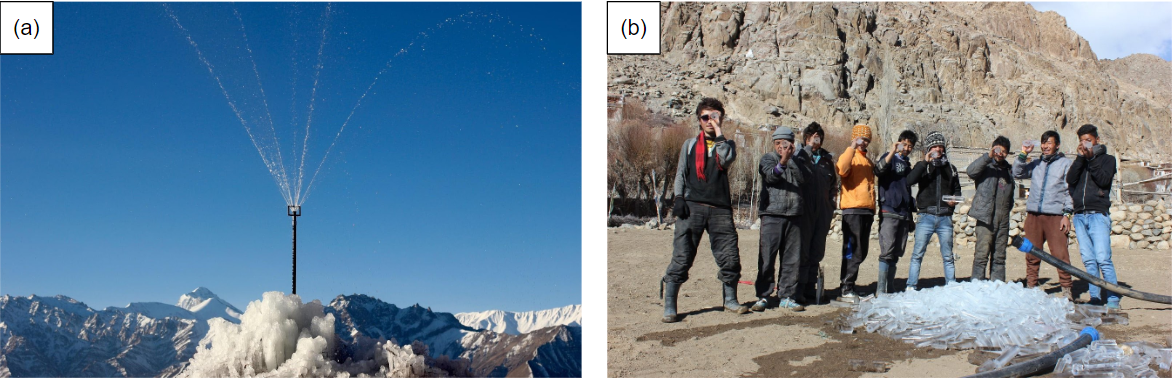
\includegraphics[width=\textwidth]{figs/construction_issues}

  \caption{The present scenario of ice stupa construction is plagued with two major issues. (a) Fountains are
  supplied with too much water. (b) Fountain discharge is interrupted frequently due to ice blocks freezing
  inside the pipeline. (Photos: Icestupa Project)}

	\label{fig:issues}
\end{figure}

\textbf{Future scenario}

In the future scenario, the automation system developed in the \textit{Technology} chapter reduces the water
consumption of each ice stupa from $60\,l/min$ to $30\,l/min$. The additional cost to install such a system was
around thousand dollars. This enabled two farmers to build 8 ice stupas spending less than a week of effort
since there were no pipeline freezing events to deal with (Fig. \ref{fig:icestupa_valley}). The total ice
volumes frozen, however, resulted in more than two times higher irrigation water supply from mid-April to
mid-June.

\begin{figure}[htb]
	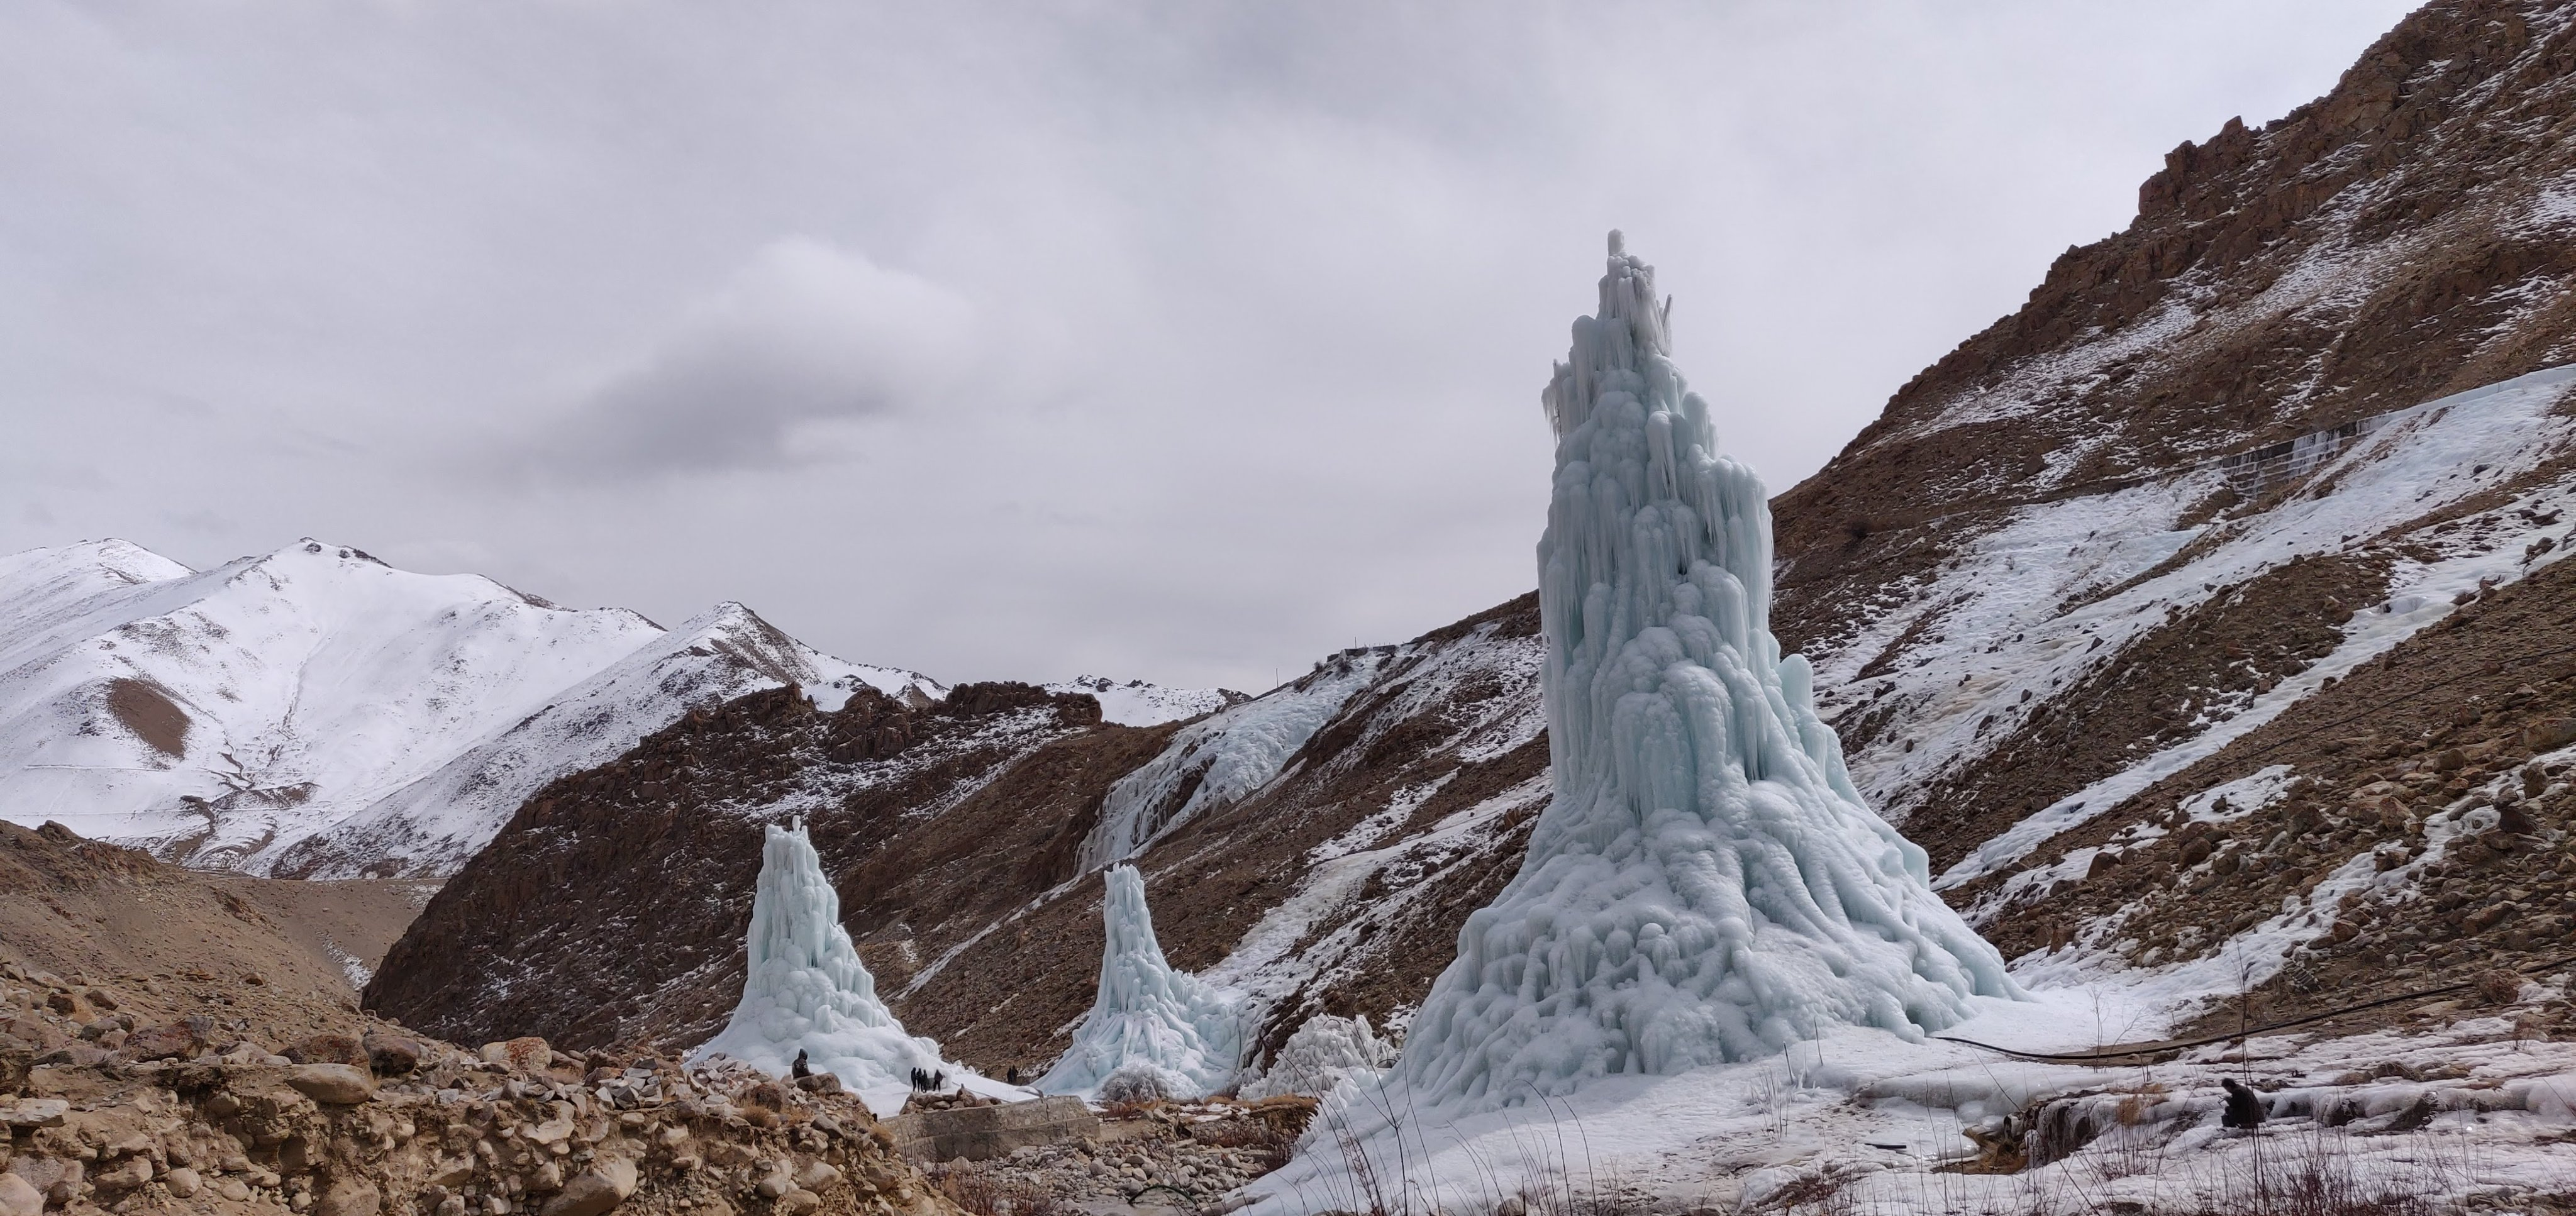
\includegraphics[width=\textwidth]{figs/icestupa_valley}

  \caption{More than a month of effort from a dozen farmers were required to build five ice stupas across the
  Gangles valley in the winter of 2019/20. This research provides tools that two farmers can leverage to
  guarantee two times more winter water storage and reduce maintenance requirements to just a few days. (Photo:
  S. Balasubramanian)}

	\label{fig:icestupa_valley}
\end{figure}

\section{Conclusions}

Glaciers provide an important buffer for highly seasonal precipitation regimes
\citep{kaserContributionPotentialGlaciers2010}. Under the currently available climate change projections it is
expected that glacial mass loss will continue in future decades, and that several smaller glaciers will continue
to disappear completely \citep{rabatelCurrentStateGlaciers2013}.

These trends stress the importance of increased water storage capacity for glacierized catchments as a pathway
for climate adaptation. Because of the challenges and cost related to traditional storage efforts, \ac{AIRs} can
be a better tool to adapt against reduced glacial runoff. In order to quantify their adaptation potential, it is
necessary to understand the volume dynamics of AIR melting, but also map how their meltwater contributes to
current and future water use. 

In this thesis, the volume variations among eighteen \ac{AIRs} were studied and their corresponding magnitudes
were explained in terms of the influence of the chosen location's meteorology, topography and the construction
strategy used. Three energy and mass balance models were used to simulate AIR evolution using data from field
measurements in Gangles, India and Guttannen, Switzerland. The use of these data sets, in combination with the
models, allowed for an accurate representation of the complex evolution that is typical of an AIR.  Although the
approach is demonstrated on specific locations, it can be extended using the open-sourced models and global
reanalysis data sets to account for spatio-temporal meteorological influences of future locations on AIR's
volume dynamics. Our main conclusions are summarized below:

\begin{figure}[htb]
  \centering
	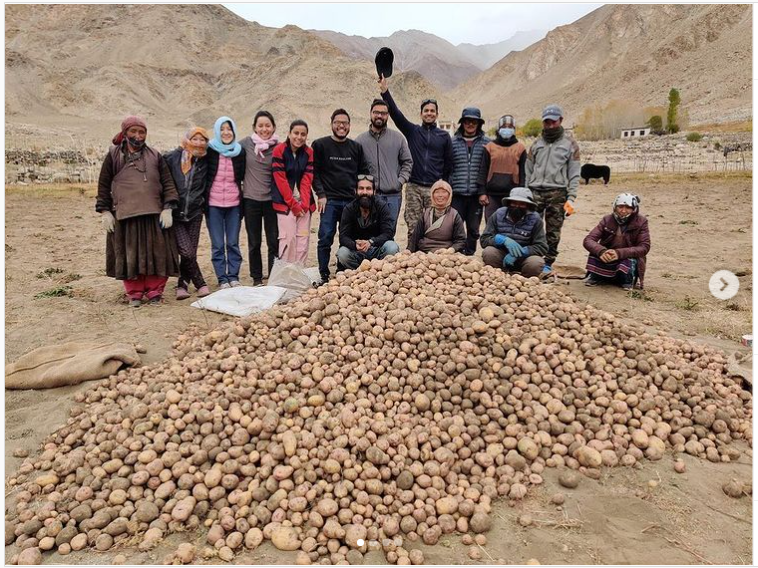
\includegraphics[width=8 cm]{figs/Kullum_potatoes}
	\caption{One of the deserted villages in Ladakh where AIR meltwater supported a harvest of 1300 kg of
		potatoes in October 2021. (Photo: Icestupa Project)}
	\label{fig:kullum_potatoes}
\end{figure}

\begin{enumerate}

  \item The Indian construction site produced long-lasting \ac{AIRs} with four times higher maximum ice volumes
    since it was colder, drier and less cloudy compared to the Swiss construction site. Thus, the \ac{AIR}
    technology is ideally suited to serve as a water management strategy, especially in dry and cold mountain
    catchments such as in \ac{HMA} or the Andes.

  \item Water losses of ice stupas were observed to be upto 80 \% due to excessive water input. However, the use
    of automated fountain scheduling strategies can lower their water consumption upto 10 times while reducing
    their maintenance requirements.

\end{enumerate}

While the spatiotemporal dynamics of AIR melt are increasingly well understood and documented in this thesis,
major uncertainty remains on how their meltwater contribution propagates through the hydrological system and
compares against the total discharge of mountain catchments. Future research needs to determine which catchments
can benefit most from the supplementary water supply by these ice harvesting technologies and provide tools that
upscale their meltwater supply.

% Model development is an art where subjective choices seek a balance between a model's simplicity
% and its accuracy.
